\documentclass[12pt]{article}
\usepackage{tikz}
\usepackage{pgfplots}
\usepackage{amsmath}
\usepackage{amsfonts}
\begin{document}
\title{Electrical Engineering 102, Homework 7}
\date{December 6th, 2018}
\author{Michael Wu\\UID: 404751542}
\maketitle

\section*{Problem 1}

\paragraph{a)}

The Nyquist rate of this signal is \(5\) Hz. The cutoff frequency of the low pass filter is \(2.5\) Hz.

\paragraph{b)}

If we sample with a frequency of \(2\) Hz, this corresponds to convolution in the frequency domain with an impulse train of
period \(4\pi\). If we sample with a frequency of \(2.5\) Hz, this corresponds to convolution in the frequency domain with
an impulse train of period \(5\pi\). Thus for the \(2\) Hz sample rate, we obtain a spectrum as shown below.
\begin{center}
    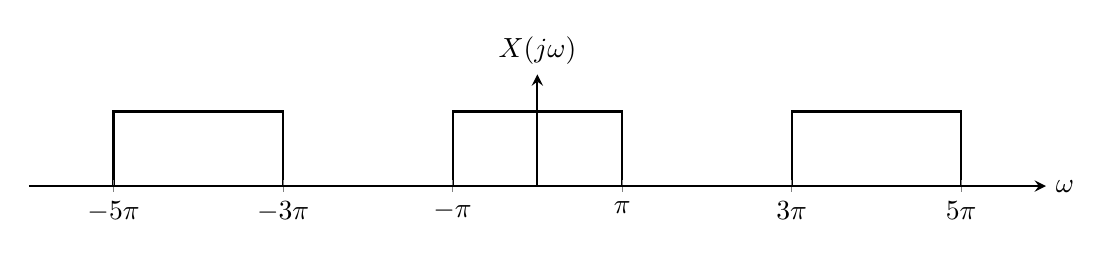
\begin{tikzpicture}
        \begin{axis}[
            axis line style=thick,
            axis lines=middle, enlargelimits=true, xlabel=\(\omega\), ylabel=\(X(j\omega)\),
            every axis y label/.style={at=(current axis.above origin),anchor=south},
            every axis x label/.style={at=(current axis.right of origin),anchor=west},
            height=3cm, width=14.5cm,
            xtick={-5,-3,-1,1,3,5},
            xticklabels={\(-5\pi\), \(-3\pi\), \(-\pi\), \(\pi\), \(3\pi\), \(5\pi\)},
            ytick=\empty,
            ymin=0, ymax=1.5,
            xmin=-6, xmax=6,
            enlargelimits=false, clip=false, axis on top,
            grid = none
        ]
            \addplot[color=black,style=thick,mark=none] coordinates {
                (-5,0)
                (-5,1)
                (-3,1)
                (-3,0)
                (-1,0)
                (-1,1)
                (1,1)
                (1,0)
                (3,0)
                (3,1)
                (5,1)
                (5,0)
            };
        \end{axis}
    \end{tikzpicture}
\end{center}
For the \(2.5\) Hz sample rate, we obtain a spectrum as shown below.
\begin{center}
    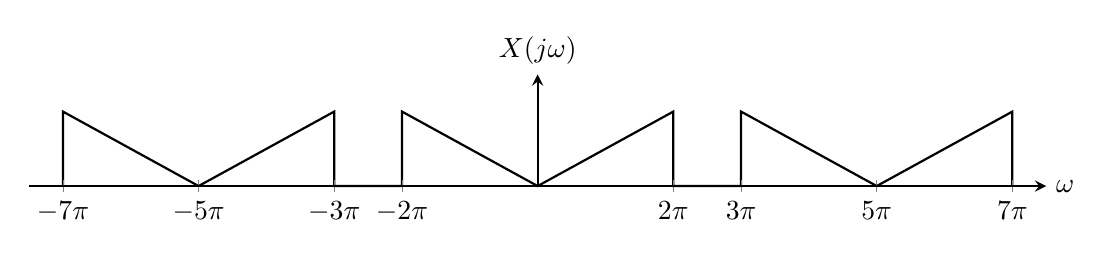
\begin{tikzpicture}
        \begin{axis}[
            axis line style=thick,
            axis lines=middle, enlargelimits=true, xlabel=\(\omega\), ylabel=\(X(j\omega)\),
            every axis y label/.style={at=(current axis.above origin),anchor=south},
            every axis x label/.style={at=(current axis.right of origin),anchor=west},
            height=3cm, width=14.5cm,
            xtick={-7,-5,-3,-2,2,3,5,7},
            xticklabels={\(-7\pi\), \(-5\pi\), \(-3\pi\), \(-2\pi\), \(2\pi\), \(3\pi\), \(5\pi\), \(7\pi\)},
            ytick=\empty,
            ymin=0, ymax=1.5,
            xmin=-7.5, xmax=7.5,
            enlargelimits=false, clip=false, axis on top,
            grid = none
        ]
            \addplot[color=black,style=thick,mark=none] coordinates {
                (-7,0)
                (-7,1)
                (-5,0)
                (-3,1)
                (-3,0)
                (-2,0)
                (-2,1)
                (0,0)
                (2,1)
                (2,0)
                (3,0)
                (3,1)
                (5,0)
                (7,1)
                (7,0)
            };
        \end{axis}
    \end{tikzpicture}
\end{center}
Thus we should use the \(2.5\) Hz sample rate with a bandpass filter that has a lower cutoff frequency of \(1.5\) Hz and an upper cutoff frequency of \(2.5\) Hz. Based
on the diagrams shown above, the only frequencies below the Nyquist rate that we can successfully sample at lie in the range of \(2.5\) Hz to \(3\) Hz. Thus the
lowest frequency at which we can sample and still recover the original signal is \(2.5\) Hz.

\section*{Problem 2}

\paragraph{a)}

\[f(t)=\delta_2(t)+\delta_2(t-1-\tau)\]

\paragraph{b)}

\begin{align*}
    F(j\omega)&=\pi\delta_\pi(\omega)+\pi\delta_\pi(\omega)e^{-j\omega(1+\tau)}\\
    &=\pi\delta_\pi(\omega)\left(1+e^{-j\omega(1+\tau)}\right)
\end{align*}

\paragraph{c)}

At \(\tau=0\), we have the following expression
\begin{align*}
    F(j\omega)&=\pi\delta_\pi(\omega)(1+e^{-j\omega})\\
    &=\pi\sum_{k=-\infty}^\infty \delta(\omega-k\pi)(1+e^{-j\omega})\\
    &=\pi\sum_{k=-\infty}^\infty \delta(\omega-k\pi)(1+e^{-jk\pi})\\
    &=\pi\sum_{k=-\infty}^\infty \delta(\omega-k\pi)(1+(-1)^k)\\
    &=\pi\sum_{k=-\infty}^\infty 2\delta(\omega-2k\pi) + 0\delta(\omega-(2k+1)\pi)\\
    &=2\pi\delta_{2\pi}(\omega)
\end{align*}
which is exactly the Fourier transform of \(\delta_1(t)\).

\section*{Problem 3}

\paragraph{a)}

\begin{enumerate}
    \item First note that
    \[(\sin(\omega_0 t))^2 = \frac{1-\cos(2\omega_0 t)}{2}\]
    Which has the Laplace transform
    \begin{align*}
        \mathcal{L}\left[(\sin(\omega_0 t)^2\right]&=\mathcal{L}\left[\frac{1-\cos(2\omega_0 t)}{2}\right]\\
        &=\frac{1}{2}\left(\frac{1}{s}-\frac{s}{s^2+(2\omega_0)^2}\right)\\
        &=\frac{2\omega_0^2}{s^3+4s\omega_0^2}
    \end{align*}
    Then by applying the frequency shift property we obtain the following.
    \[\mathcal{L}\left[e^{-at}(\sin(\omega_0 t))^2\right]=\frac{2\omega_0^2}{(s+a)^3+4(s+a)\omega_0^2}\]
    Then by applying the multiplication by \(t\) rule we obtain the following.
    \[\mathcal{L}\left[te^{-at}(\sin(\omega_0 t))^2\right]=\frac{2\omega_0^2(3(s+a)^2+4\omega_0^2)}{((s+a)^3+4(s+a)\omega_0^2)^2}\]
    Since the region of convergence of \(\mathcal{L}[1]\) and \(\mathcal{L}[\cos(2\omega_0 t)]\) is for \(\mathbb{R}(s)>0\) and we shift our Laplace
    transform by \(-a\), the region of convergence for this Laplace transform is for \(\mathbb{R}(s+a)>0\).
    \item The Laplace transform of this function is the following.
    \begin{align*}
        \mathcal{L}[f(t)] &= \int_1^2 e^{-st}\,dt + \int_2^\infty e^6e^{-(s+2)t}\,dt\\
        &=\left.-\frac{e^{-st}}{s}\right|_1^2 + \left.-\frac{e^6e^{-(s+2)t}}{s+2}\right|_2^\infty\\
        &=\frac{e^{-s}-e^{-2s}}{s} + \frac{e^6e^{-(s+2)2}}{s+2}\\
        &=\frac{e^{-s}(1-e^{-s})}{s} + \frac{e^{-2s+2}}{s+2}
    \end{align*}
    This has a region of convergence of \(\mathbb{R}(s+2)>0\), due to the \(s+2\) term in the right integral term.
    \item The Laplace transform of this function is the following.
    \begin{align*}
        \mathcal{L}[f(t)] &= \int_0^1 \sin(2\pi t)e^{-st}\,dt\\
        &=\int_0^1 \frac{e^{j2\pi t}-e^{-j2\pi t}}{2j}e^{-st}\,dt\\
        &=\int_0^1 \frac{e^{(-s+j2\pi) t}-e^{(-s-j2\pi) t}}{2j}\,dt\\
        &=\left.\frac{e^{(-s+j2\pi) t}}{2j(-s+j2\pi)}\right|_0^1-\left.\frac{e^{(-s-j2\pi) t}}{2j(-s-j2\pi)}\right|_0^1\\
        &=\frac{e^{(-s+j2\pi)}-1}{2j(-s+j2\pi)}-\frac{e^{(-s-j2\pi)}-1}{2j(-s-j2\pi)}\\
        &=\frac{e^{-s}-1}{2j(-s+j2\pi)}-\frac{e^{-s}-1}{2j(-s-j2\pi)}\\
        &=-\frac{(e^{-s}-1)(-2js+4\pi) - (e^{-s}-1)(-2js-4\pi)}{4(s^2+4\pi^2)}\\
        &=-\frac{8\pi(e^{-s}-1)}{4(s^2+4\pi^2)}\\
        &=\frac{2\pi-2\pi e^{-s}}{s^2+4\pi^2}
    \end{align*}
\end{enumerate}

\paragraph{b)}

\begin{enumerate}
    \item This can be obtained from \(X(s)\) since we can use the frequency shifting rule to find the Laplace transform of \(x(t)e^{-t}\). The region of convergence
    of this new Laplace transform would be \(\mathbb{R}(s+2)>0\) which includes the \(j\) axis. The Fourier transform is simply \(X(1+j\omega)\), which is evaluated as
    follows.
    \begin{align*}
        X(1+i\omega)&=\frac{1}{(1+j\omega)^2+2(1+j\omega)+5}\\
        &=\frac{1}{1+j2\omega-\omega^2+2+j2\omega+5}\\
        &=\frac{1}{-\omega^2+j4\omega + 8}
    \end{align*}
    \item This cannot be obtained from \(X(s)\) since after applying the frequency shifting rule, we obtain a new Laplace transform with a region of convergence of \(\mathbb{R}(s-2)>0\).
    This does not include the \(j\) axis.
\end{enumerate}

\section*{Problem 4}

\paragraph{a)}

Let us perform partial fraction decomposition, ignoring the \(e^{-s}\) term. We must solve the following.
\[A(s-2)^2 + B(s-2)(s-3) + C(s-3) = s+1\]
If we set \(s=2\), we get \(C=-3\). If we set \(s=3\), we get \(A=4\). Then if we set \(s=4\), we get
\[4A+2B+C=2B+16-3=5\]
Thus we get \(B=-4\), and our partial fraction decomposition is
\[\frac{s+1}{(s-2)^2(s-3)}=\frac{4}{s-3}-\frac{4}{s-2}-\frac{3}{(s-2)^2}\]
This is the Laplace transform of the function
\[u(t)(4e^{3t}-4e^{2t}-3te^{2t})\]
Using the time shift property to account for the \(e^{-s}\) term, the inverse Laplace transform of \(F(s)\) is
\[f(t)=u(t-1)\left(4e^{3(t-1)}-4e^{2(t-1)}-3te^{2(t-1)}\right)\]

\paragraph{b)}

In order to perform partial fraction decomposition, we must solve the following.
\[A(s^2+4) + Bs^2 + Cs = s+4\]
If we set \(s=0\), we obtain \(A=1\). If we set \(s=1\), we obtain \(B+C=0\). If we set \(s=2\), we obtain \(4B+2C=-2\). Solving these two equations yields \(B=-1\) and \(C=1\). Then
we have the decomposition
\[\frac{1}{s}+\frac{-s+1}{s^2+4}\]
This has an inverse Laplace transform of
\[f(t)=u(t)\left(1-\cos(2t)+\frac{\sin(2t)}{2}\right)\]

\paragraph{c)}

In order to perform partial fraction decomposition, we must solve the following.
\[A(s^2+2s+2) + B(s+1)(s+1-j) + C(s+1)(s+1+j) = 1\]
If we set \(s=-1\), we obtain \(A=1\). If we set \(s=-1+j\), we obtain \(C=-\frac{1}{2}\). If we set \(s=-1-j\), we obtain \(B=-\frac{1}{2}\). Then we have the decomposition
\[\frac{1}{s+1}-\frac{1}{2(s+1+j)}-\frac{1}{2(s+1-j)}\]
This has an inverse Laplace transform of
\[f(t)=u(t)\left(e^{-t}-\frac{e^{-(1+j)t}}{2}-\frac{e^{-(1-j)t}}{2}\right)=u(t)e^{-t}(1-\cos(t))\]

\section*{Problem 5}

\paragraph{a)}

Applying the Laplace transform to the differential equation yields a transfer function of the form
\[H_1(s)=\frac{a}{s^2+3s+2}\]
We can solve for \(a\) by plugging in \(x(t)=e^t\) and \(y(t)=\frac{e^t}{2}\) into the differential equation. This yields
\[\frac{1}{2}e^t+\frac{3}{2}e^t+e^t = ae^t\]
and so we obtain \(a=3\). Thus our transfer function is
\[H_1(s)=\frac{3}{(s+1)(s+2)}\]

\paragraph{b)}

When the input is \(u(t)\), we know the Laplace transform of \(y(t)\) is
\[\frac{3}{s(s+1)(s+2)}\]
Using partial fraction decomposition we can rewrite this as
\[\frac{3}{2s}-\frac{3}{s+1}+\frac{3}{2(s+2)}\]
which has an inverse Laplace transform of
\[y(t)=u(t)\left(\frac{3}{2}-3e^{-t}+\frac{3}{2}e^{-2t}\right)\]

\paragraph{c)}

In order to find the impulse response of \(S_2\), we must solve
\[(u(t)-u(t-1))*h_2(t)=r(t)-2r(t-1)+r(t-2)\]
We know that \(u(t-t_0)*u(t-t_1) = r(t-t_0-t_1)\), so if we let \(h_2(t)=u(t)-u(t-1)\) then we get
\begin{align*}
    (u(t)-u(t-1))*h_2(t)&=(u(t)-u(t-1))*(u(t)-u(t-1))\\
    &=r(t)-r(t-1)-r(t-1)+r(t-2)\\
    &=r(t)-2r(t-1)+r(t-2)
\end{align*}
Then we can find the impulse response of \(S_1\) by using the transfer function. When the input is \(\delta(t)\), the Laplace transform of \(y(t)\) is
\[\frac{3}{(s+1)(s+2)}\]
which has a partial fraction decomposition of
\[\frac{3}{s+1}-\frac{3}{s+2}\]
giving an impulse response of
\[h_1(t)=u(t)(3e^{-t}-3e^{-2t})\]
Notice that this is exactly the derivative of the step response that we found earlier. Then the total impulse response is equal to \(h(t)=h_1(t)*h_2(t)\),
which can be found as follows.
\begin{align*}
    h(t)&=h_1(t)*h_2(t)\\
    &=(u(t)(3e^{-t}-3e^{-2t}))*(u(t)-u(t-1))\\
    &=u(t)\int_0^t (3e^{-\tau}-3e^{-2\tau})\,d\tau-u(t-1)\int_0^{t-1}(3e^{-\tau}-3e^{-2\tau})\,d\tau\\
    &=u(t)\left.\left(-3e^{-\tau}+\frac{3}{2}e^{-2\tau}\right)\right|_0^t-u(t-1)\left.\left(-3e^{-\tau}+\frac{3}{2}e^{-2\tau}\right)\right|_0^{t-1}\\
    &=u(t)\left(-3e^{-t}+\frac{3}{2}e^{-2t}+\frac{3}{2}\right)-u(t-1)\left(-3e^{-(t-1)}+\frac{3}{2}e^{-2(t-1)}+\frac{3}{2}\right)
\end{align*}

\section*{Problem 6}

\paragraph{a)}

The Laplace transform of the step response is
\[\frac{1}{s(s+1)}\]
Using partial fraction decomposition, this is equal to
\[\frac{1}{s}-\frac{1}{s+1}\]
which means we can take the inverse Laplace transform to get the step response
\[y(t)=u(t)(1-e^{-t})\]
This looks like the following graph.
\begin{center}
    \begin{tikzpicture}
        \begin{axis}[
            no markers, domain=0:6, samples=500,
            axis line style=thick,
            axis lines=middle, enlargelimits=true, xlabel=\(t\), ylabel=\(y(t)\),
            every axis y label/.style={at=(current axis.above origin),anchor=south},
            every axis x label/.style={at=(current axis.right of origin),anchor=west},
            height=5cm, width=14.5cm,
            xtick distance={1},
            ytick distance={1},
            ymin=0, ymax=1.5,
            xmin=-0.5, xmax=5.99,
            enlargelimits=false, clip=false, axis on top,
            grid = none
        ]
            \addplot [very thick,black!50!black] {(\x>0)*(1-exp(-\x))};
        \end{axis}
    \end{tikzpicture}
\end{center}

\paragraph{b)}

This system can be represented by the equation
\[a(x(t)-y(t))*(e^{-t}u(t))=y(t)\]
Taking the Laplace transform of this yields
\begin{align*}
    \mathcal{L}[y(t)]&=\frac{a}{s+1}(\mathcal{L}[x(t)]-\mathcal{L}[y(t)])\\
    \left(1+\frac{a}{s+1}\right)\mathcal{L}[y(t)]&=\frac{a}{s+1}\mathcal{L}[x(t)]\\
    \frac{a+s+1}{s+1}\mathcal{L}[y(t)]&=\frac{a}{s+1}\mathcal{L}[x(t)]\\
    \frac{\mathcal{L}[y(t)]}{\mathcal{L}[x(t)]}&=\frac{a}{a+s+1}
\end{align*}
So our transfer function is
\[H(s)=\frac{a}{a+s+1}\]

\paragraph{c)}

In order to have a time constant of \(100\) ms, we must obtain an impulse response of the form \(ce^{-10t}\). This has a Laplace transform of \(\frac{c}{s+10}\).
Thus if we let \(a=9\) and \(c=9\), we obtain the transfer function \(\frac{9}{s+10}\). Then we know that the step response has a Laplace transform of
\[\frac{9}{s(s+10)}\]
which we can rewrite using partial fraction decomposition to get
\[\frac{9}{10s}-\frac{9}{10(s+10)}\]
Then taking the inverse Laplace transform yields the step response
\[\frac{9}{10}(1-e^{-10t})\]
The following graph shows the new step response in black, with the old step response in blue.
\begin{center}
    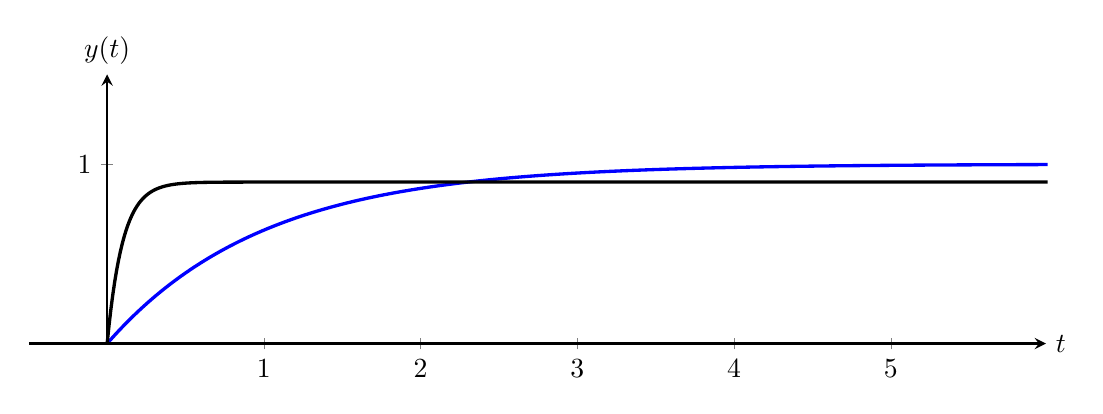
\begin{tikzpicture}
        \begin{axis}[
            no markers, domain=0:6, samples=500,
            axis line style=thick,
            axis lines=middle, enlargelimits=true, xlabel=\(t\), ylabel=\(y(t)\),
            every axis y label/.style={at=(current axis.above origin),anchor=south},
            every axis x label/.style={at=(current axis.right of origin),anchor=west},
            height=5cm, width=14.5cm,
            xtick distance={1},
            ytick distance={1},
            ymin=0, ymax=1.5,
            xmin=-0.5, xmax=5.99,
            enlargelimits=false, clip=false, axis on top,
            grid = none
        ]
            \addplot [very thick,blue!50!blue] {(\x>0)*(1-exp(-\x))};
            \addplot [very thick,black!50!black] {(\x>0)*0.9*(1-exp(-10*\x))};
        \end{axis}
    \end{tikzpicture}
\end{center}

\end{document}